%
%
% Kapitel Anhang
%
%


\appendix

\chapter{Anhang}
\refstepcounter{chapter}

\section{Verteilung der Schnittvariablen der Selektion von \texorpdfstring{$t\overline{t}+\gamma$}{ttg}-Ereignissen}
\label{sec:kontrollplots}

Im Folgenden werden die Verteilungen aller Variablen, auf die in der Selektion von {$t\overline{t}+\gamma$}-Ereignissen (Abschnitt \ref{sec:ttg_selektion}) geschnitten wird, gezeigt. Exemplarisch werden dazu die Verteilungen des Datensatzes f�r $d_A^{\gamma} = 0$ gew�hlt.

\begin{figure}%
\centering
\begin{subfigure}[b]{0.48\textwidth}
  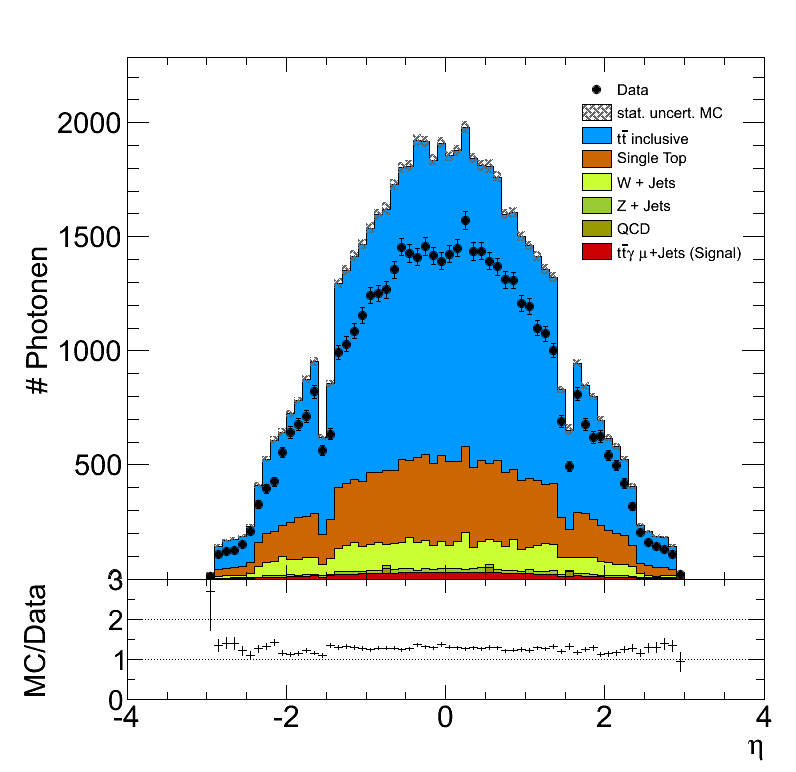
\includegraphics[width=\textwidth]{bilder/eta_linear}%
\end{subfigure}
\begin{subfigure}[b]{0.48\textwidth}
  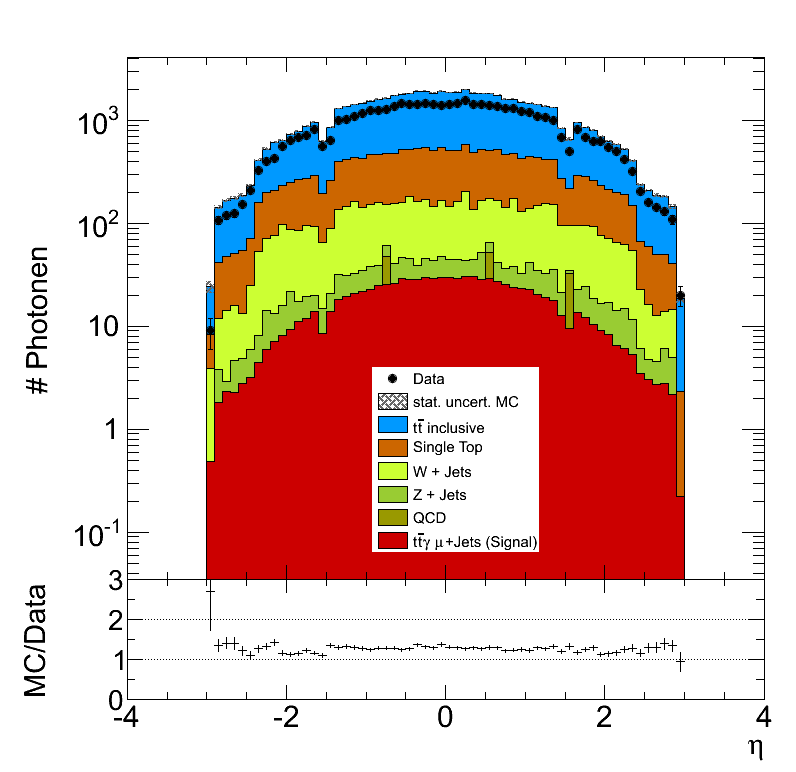
\includegraphics[width=\textwidth]{bilder/eta_log}%
\end{subfigure}
\caption{$\eta$-Verteilung des Photons in linearer (links) und halblogarithmischer (rechts) Auftragung. Forderung: $\left|\eta\right| < 1,4442$ und $1,556 < \left|\eta\right| < 2,4$.}%
\label{fig:eta_cut}%
\end{figure}

\begin{figure}%
\centering
\begin{subfigure}[b]{0.48\textwidth}
  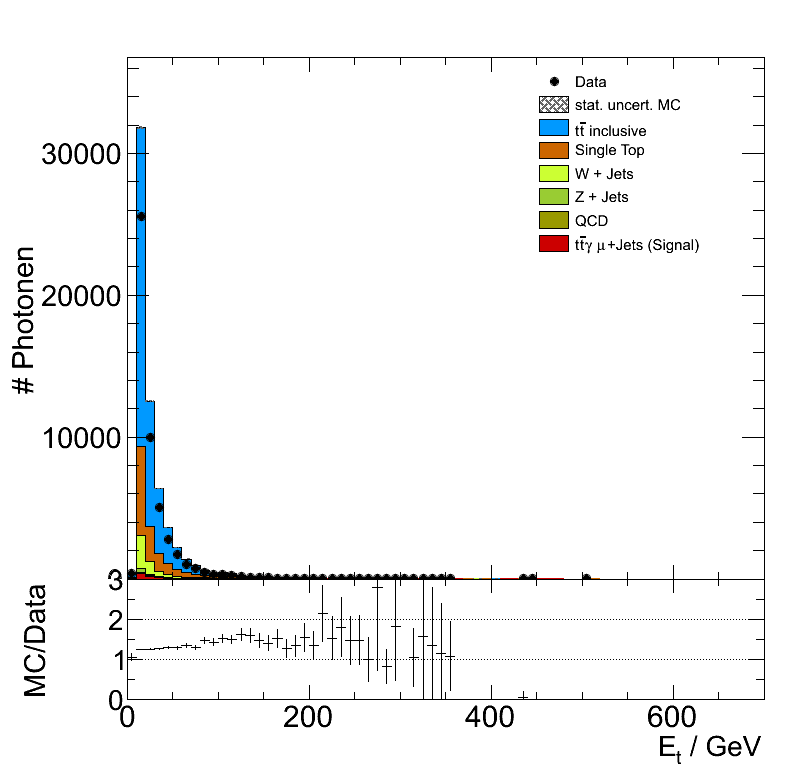
\includegraphics[width=\textwidth]{bilder/et_linear}%
\end{subfigure}
\begin{subfigure}[b]{0.48\textwidth}
  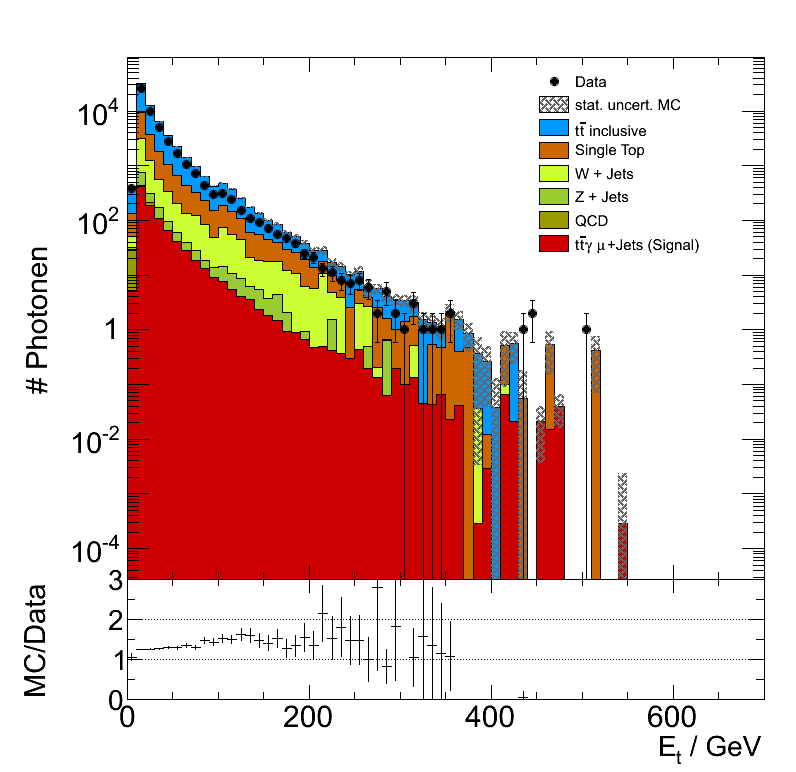
\includegraphics[width=\textwidth]{bilder/et_log}%
\end{subfigure}
\caption{$E_T$-Verteilung des Photons in linearer (links) und halblogarithmischer (rechts) Auftragung. Forderung: $E_T > 20$\,GeV.}%
\label{fig:et_cut}%
\end{figure}

\begin{figure}%
\centering
\begin{subfigure}[b]{0.48\textwidth}
  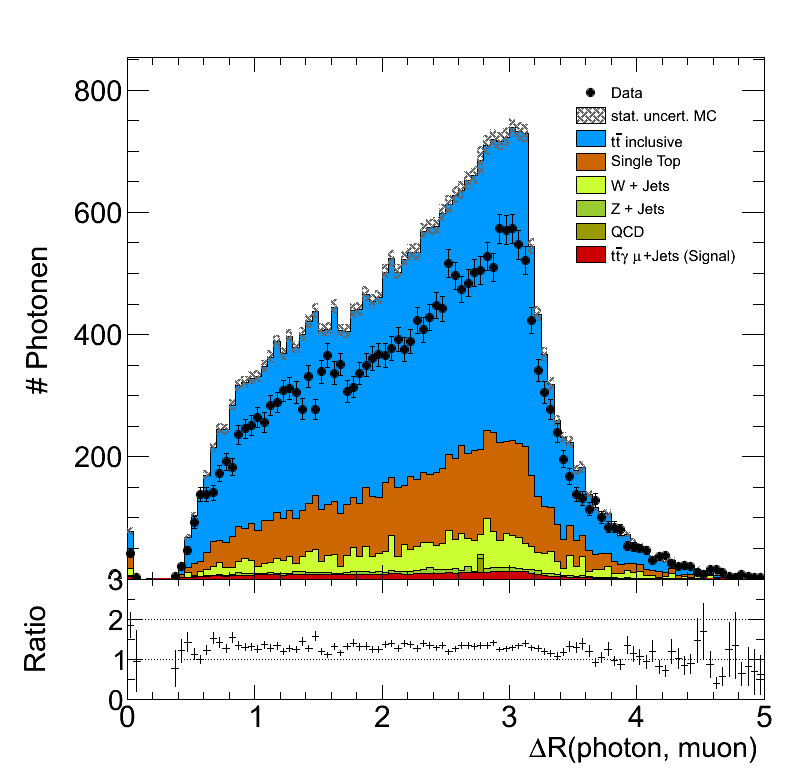
\includegraphics[width=\textwidth]{bilder/drmuon_linear}%
\end{subfigure}
\begin{subfigure}[b]{0.48\textwidth}
  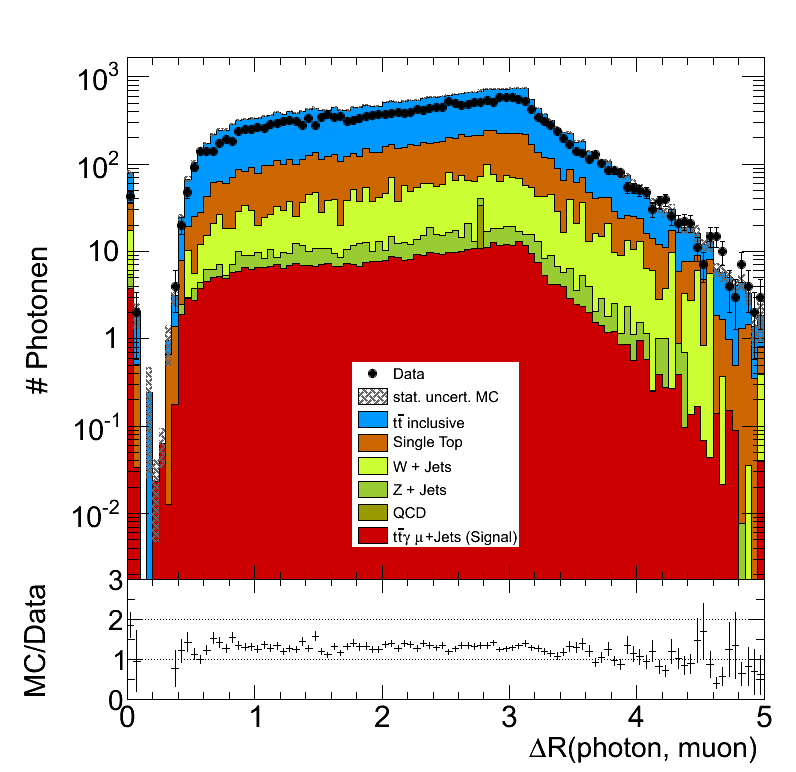
\includegraphics[width=\textwidth]{bilder/drmuon_log}%
\end{subfigure}
\caption{$\Delta R(\gamma,\mu)$-Verteilung des Photons in linearer (links) und halblogarithmischer (rechts) Auftragung. Forderung: $\Delta R(\gamma,\mu) > 0,3$.}%
\label{fig:drmuon_cut}%
\end{figure}

\begin{figure}%
\centering
\begin{subfigure}[b]{0.48\textwidth}
  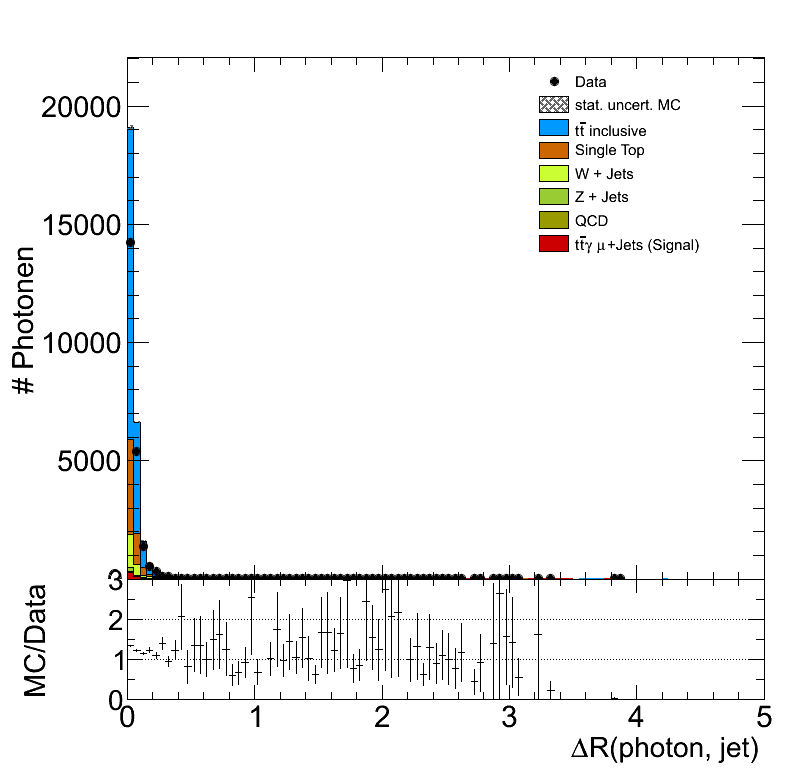
\includegraphics[width=\textwidth]{bilder/drjet_linear}%
\end{subfigure}
\begin{subfigure}[b]{0.48\textwidth}
  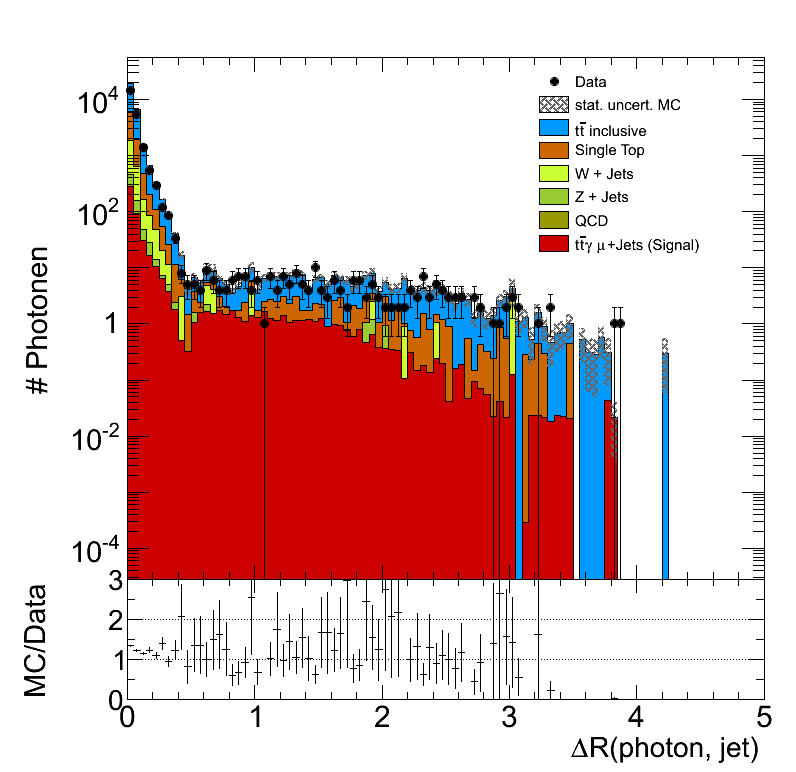
\includegraphics[width=\textwidth]{bilder/drjet_log}%
\end{subfigure}
\caption{$\Delta R(\gamma,\text{jet})$-Verteilung des Photons in linearer (links) und halblogarithmischer (rechts) Auftragung. Forderung: $\Delta R(\gamma,\text{jet}) < 0,15$ oder $\Delta R(\gamma,\text{jet}) > 0,5$.}%
\label{fig:drjet_cut}%
\end{figure}

\begin{figure}%
\centering
\begin{subfigure}[b]{0.48\textwidth}
  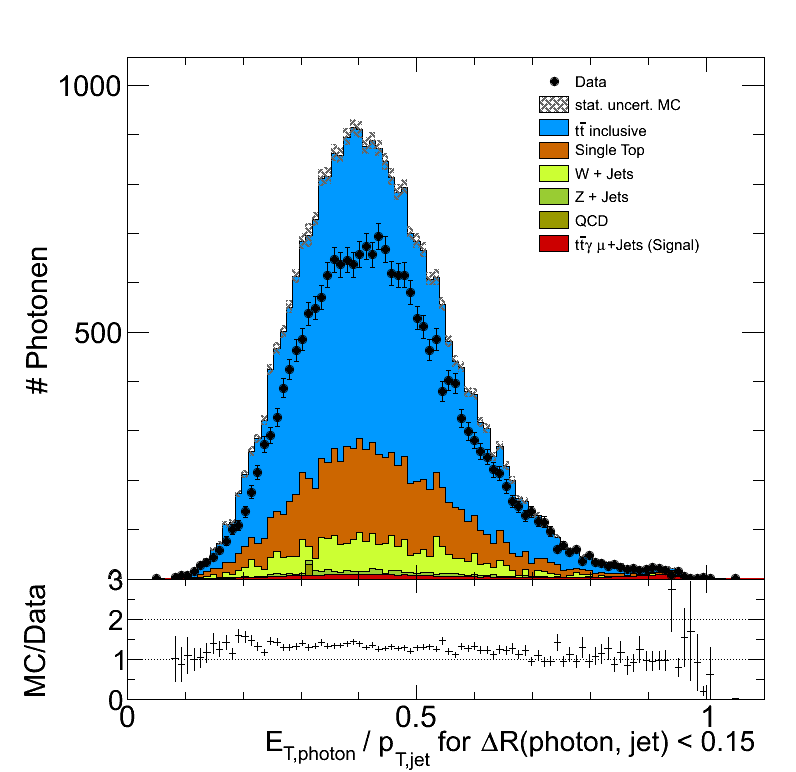
\includegraphics[width=\textwidth]{bilder/ptreldrjet_linear}%
\end{subfigure}
\begin{subfigure}[b]{0.48\textwidth}
  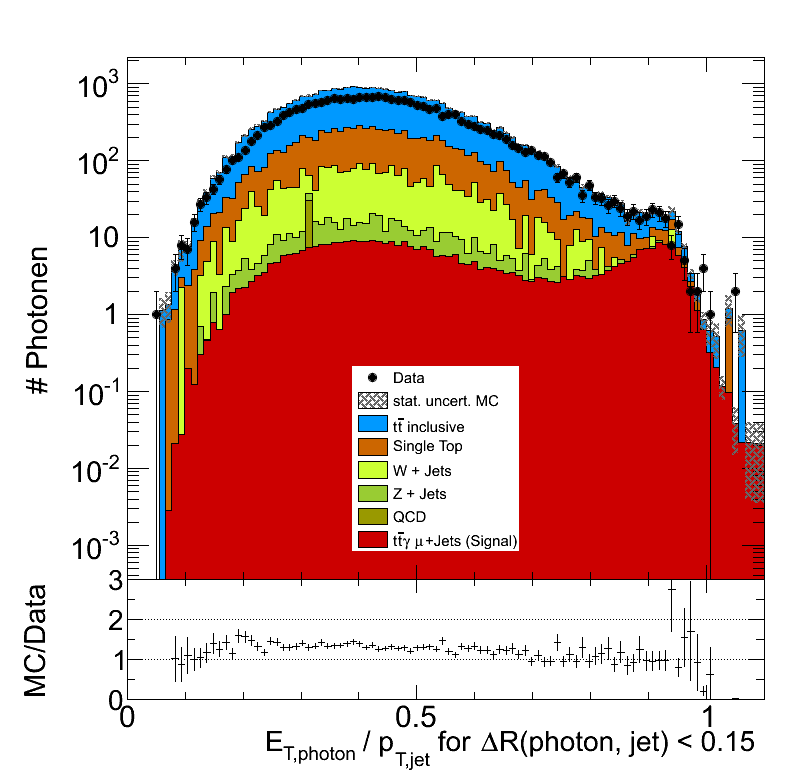
\includegraphics[width=\textwidth]{bilder/ptreldrjet_log}%
\end{subfigure}
\caption{$E_{T,\gamma}/p_{T,jet}$-Verteilung des Photons f�r Photonen innerhalb von $\Delta R(\gamma,\text{jet}<0,15$ in linearer (links) und halblogarithmischer (rechts) Auftragung. Forderung: $E_{T,\gamma}/p_{T,jet} > 0,75$.}%
\label{fig:ptreldrjet_cut}%
\end{figure}

\begin{figure}%
\centering
\begin{subfigure}[b]{0.48\textwidth}
  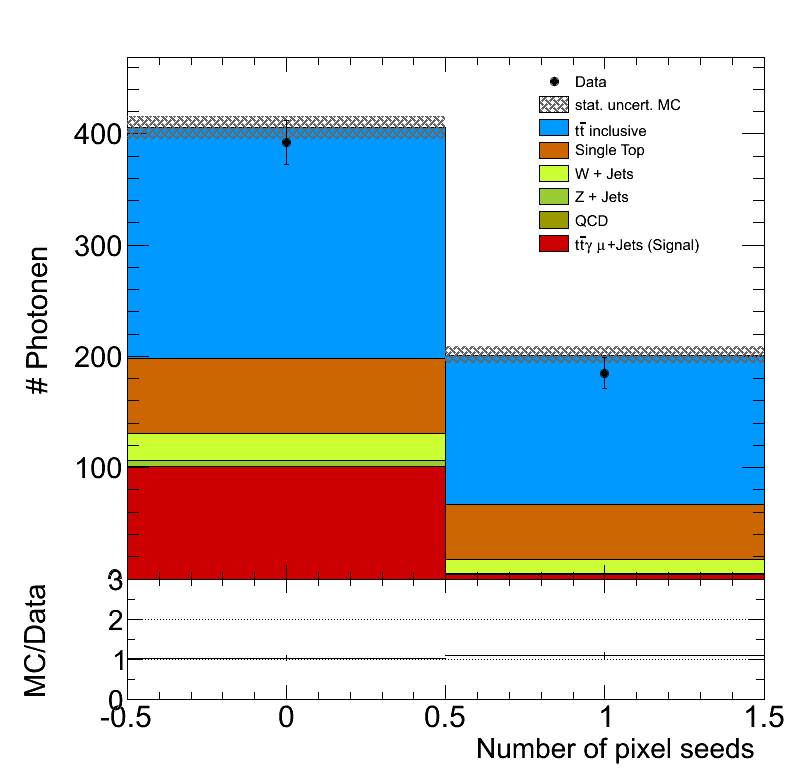
\includegraphics[width=\textwidth]{bilder/haspixelseeds_linear}%
\end{subfigure}
\begin{subfigure}[b]{0.48\textwidth}
  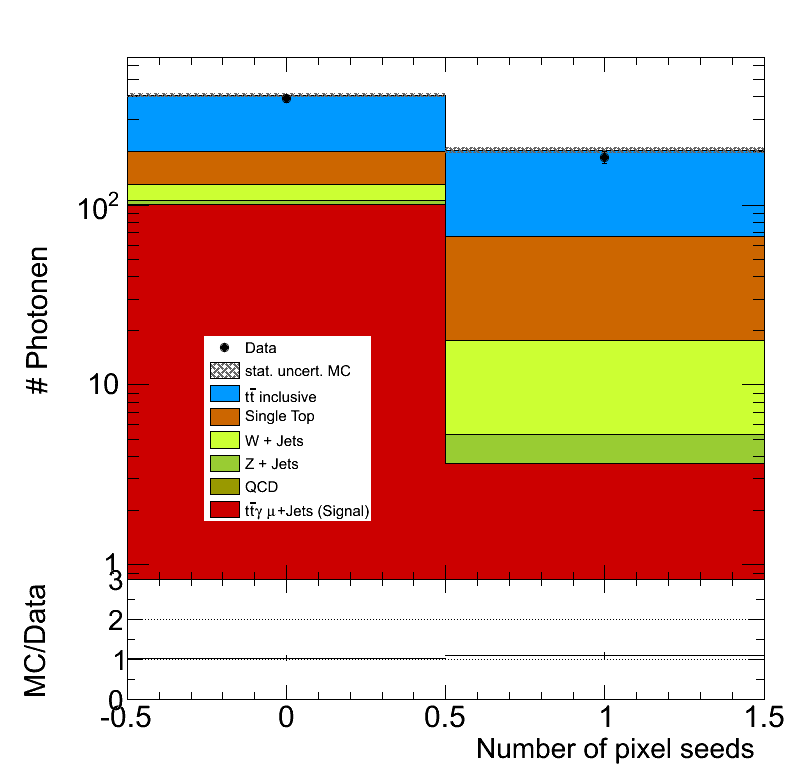
\includegraphics[width=\textwidth]{bilder/haspixelseeds_log}%
\end{subfigure}
\caption{\enquote{Has-Pixel-Seed}-Verteilung des Photons in linearer (links) und halblogarithmischer (rechts) Auftragung. Forderung: Kein pixel seed.}%
\label{fig:haspixelseeds_cut}%
\end{figure}

\begin{figure}%
\centering
\begin{subfigure}[b]{0.48\textwidth}
  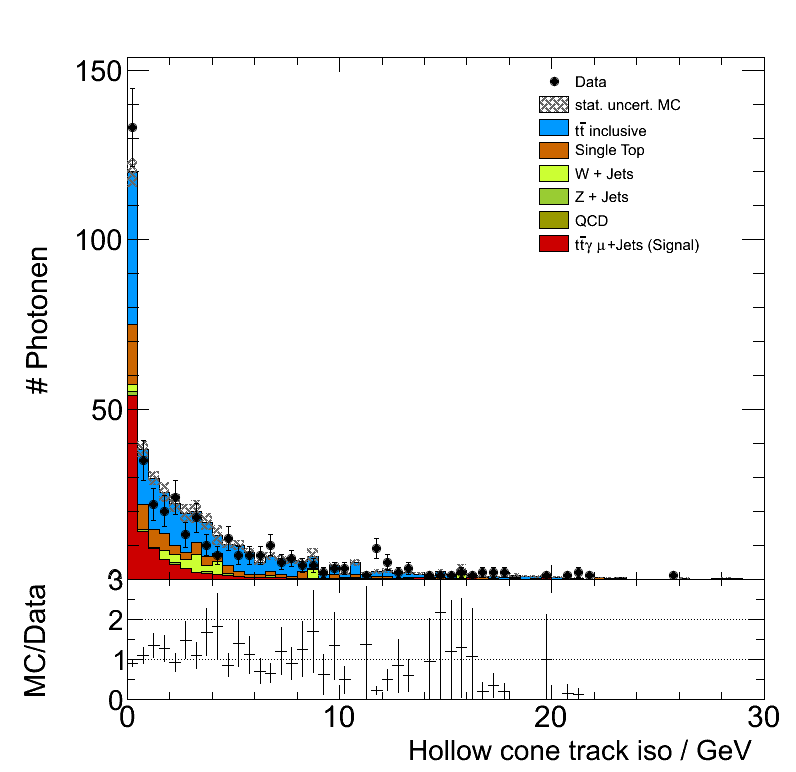
\includegraphics[width=\textwidth]{bilder/hollowconetrackiso_linear}%
\end{subfigure}
\begin{subfigure}[b]{0.48\textwidth}
  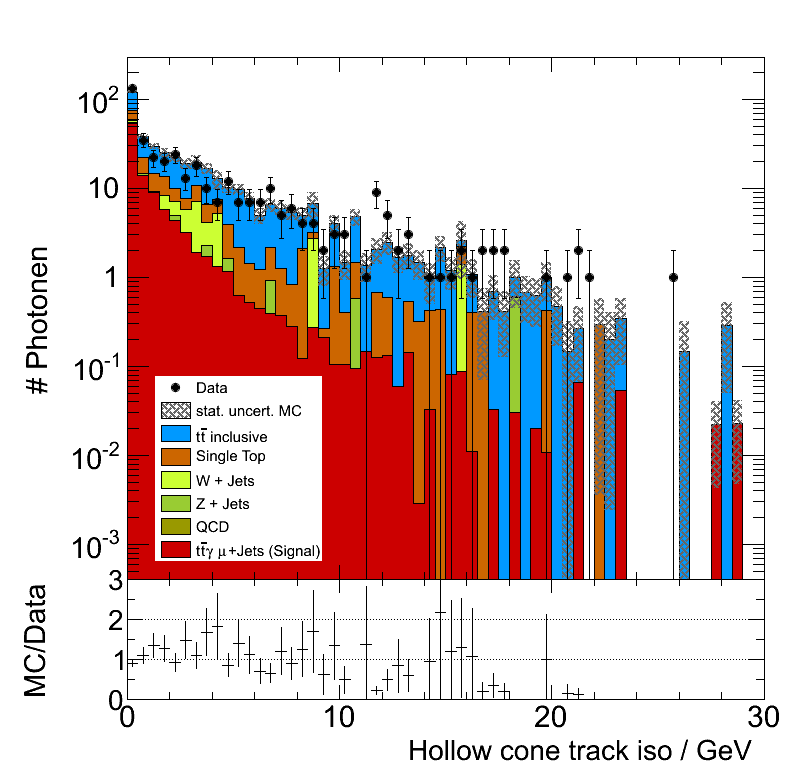
\includegraphics[width=\textwidth]{bilder/hollowconetrackiso_log}%
\end{subfigure}
\caption{Spur-Isolations-Verteilung des Photons in linearer (links) und halblogarithmischer (rechts) Auftragung. Forderung: $\Sigma_{trk} < 2,0 + 0,001\cdot E_T$.}%
\label{fig:hollowconetrackiso_cut}%
\end{figure}

\begin{figure}%
\centering
\begin{subfigure}[b]{0.48\textwidth}
  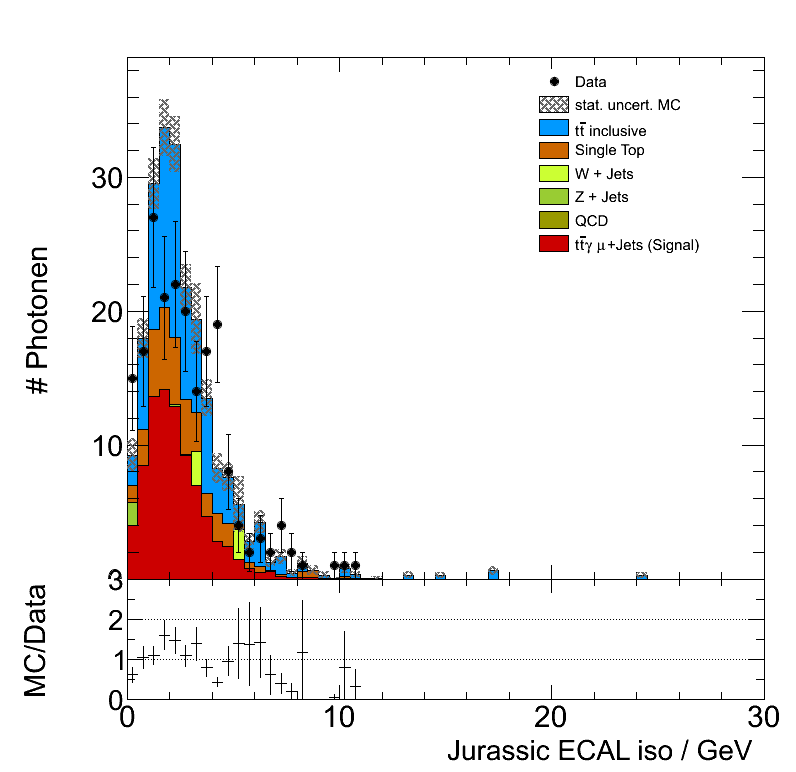
\includegraphics[width=\textwidth]{bilder/jurassicecaliso_linear}%
\end{subfigure}
\begin{subfigure}[b]{0.48\textwidth}
  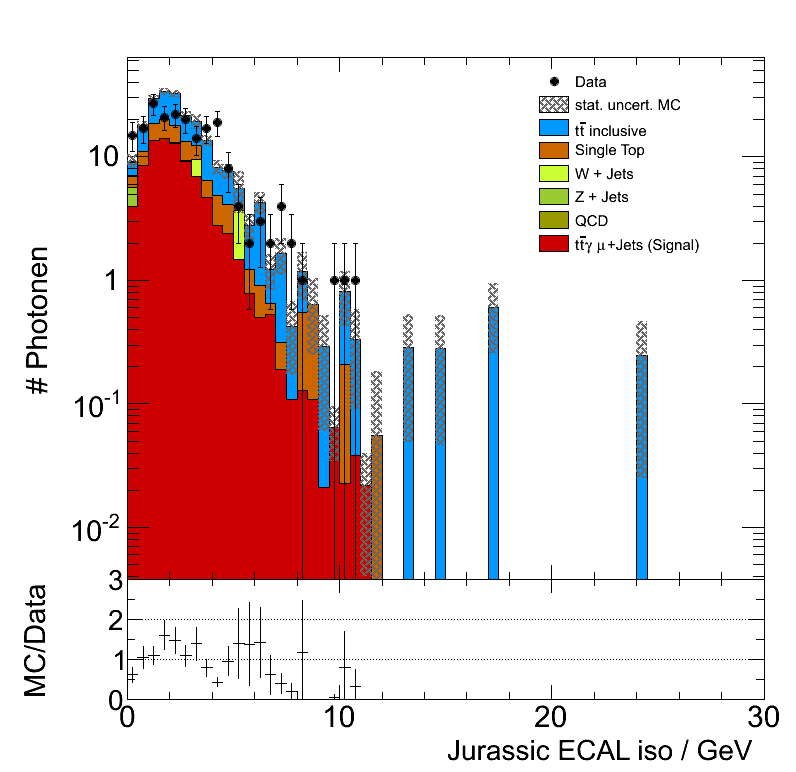
\includegraphics[width=\textwidth]{bilder/jurassicecaliso_log}%
\end{subfigure}
\caption{ECAL-Isolations-Verteilung des Photons in linearer (links) und halblogarithmischer (rechts) Auftragung. Forderung: $\Sigma_{ECAL} < 4,2 + 0,006\cdot E_T$.}%
\label{fig:jurassicecaliso_cut}%
\end{figure}

\begin{figure}%
\centering
\begin{subfigure}[b]{0.48\textwidth}
  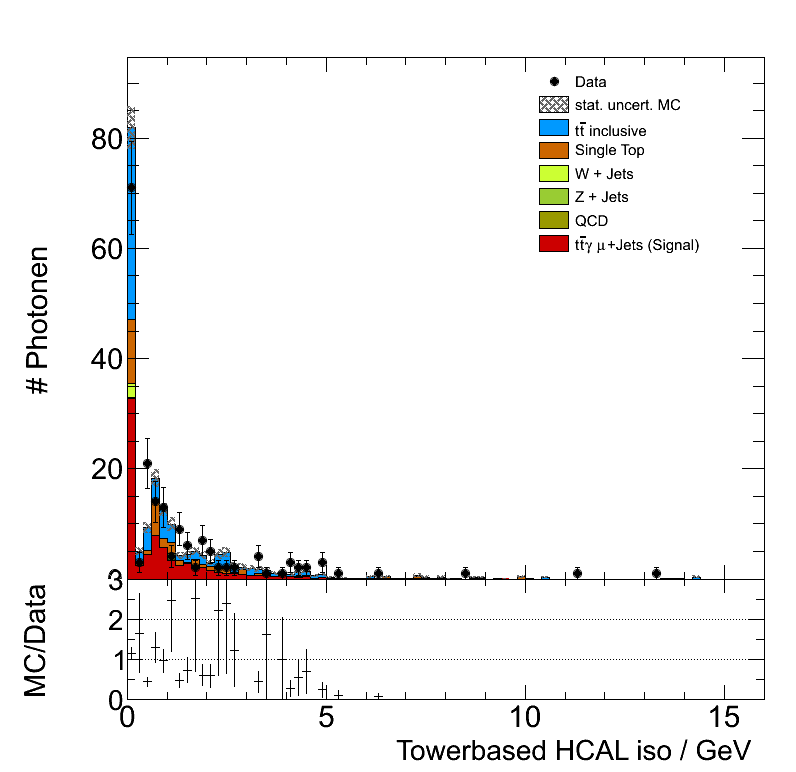
\includegraphics[width=\textwidth]{bilder/hcaliso_linear}%
\end{subfigure}
\begin{subfigure}[b]{0.48\textwidth}
  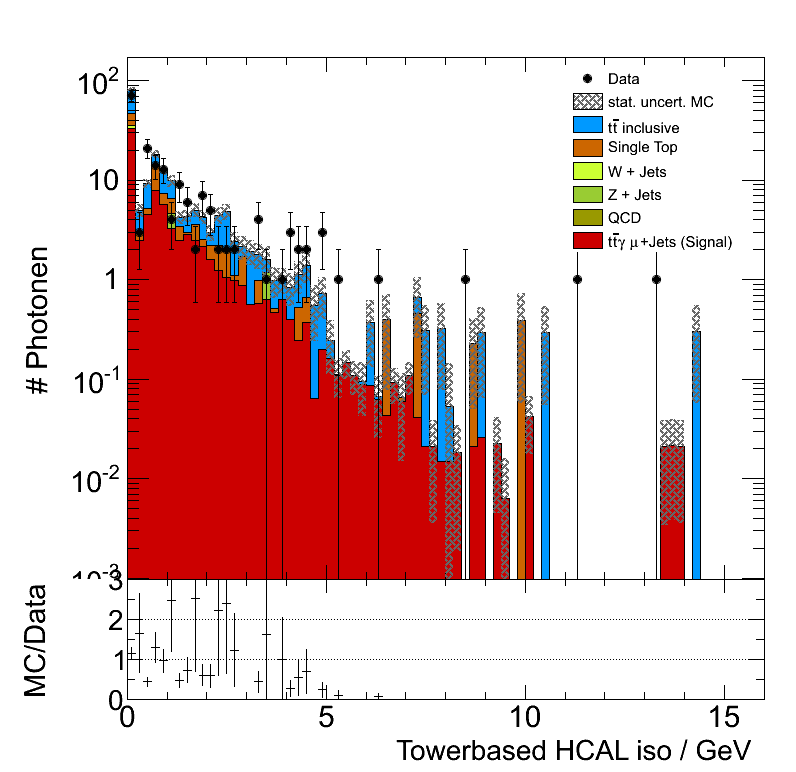
\includegraphics[width=\textwidth]{bilder/hcaliso_log}%
\end{subfigure}
\caption{HCAL-Isolations-Verteilung des Photons in linearer (links) und halblogarithmischer (rechts) Auftragung. Forderung: $\Sigma_{HCAL} < 2,2 + 0,0025\cdot E_T$.}%
\label{fig:hcaliso_cut}%
\end{figure}

\begin{figure}%
\centering
\begin{subfigure}[b]{0.48\textwidth}
  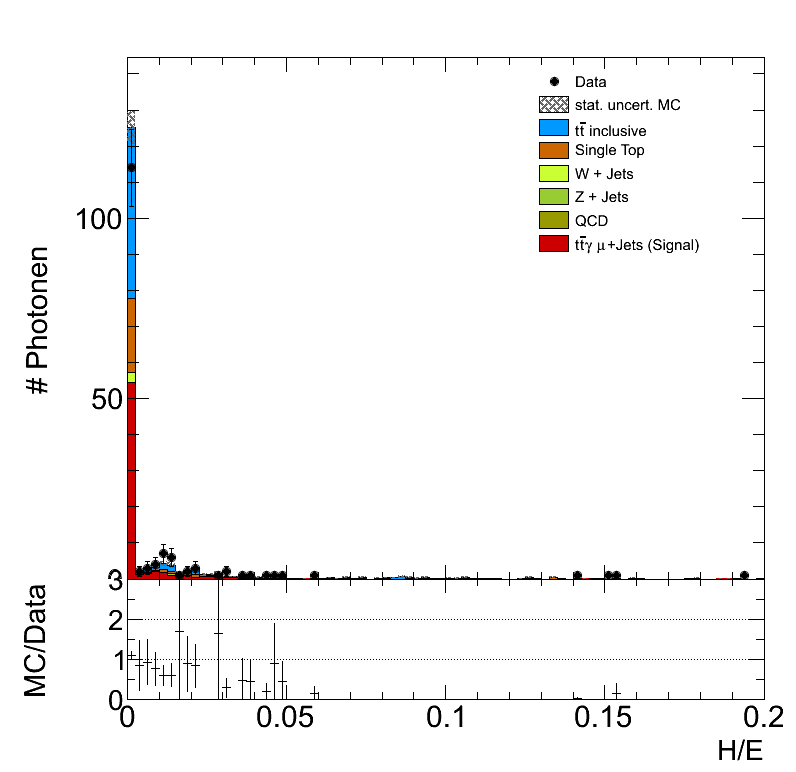
\includegraphics[width=\textwidth]{bilder/hadronicoverem_linear}%
\end{subfigure}
\begin{subfigure}[b]{0.48\textwidth}
  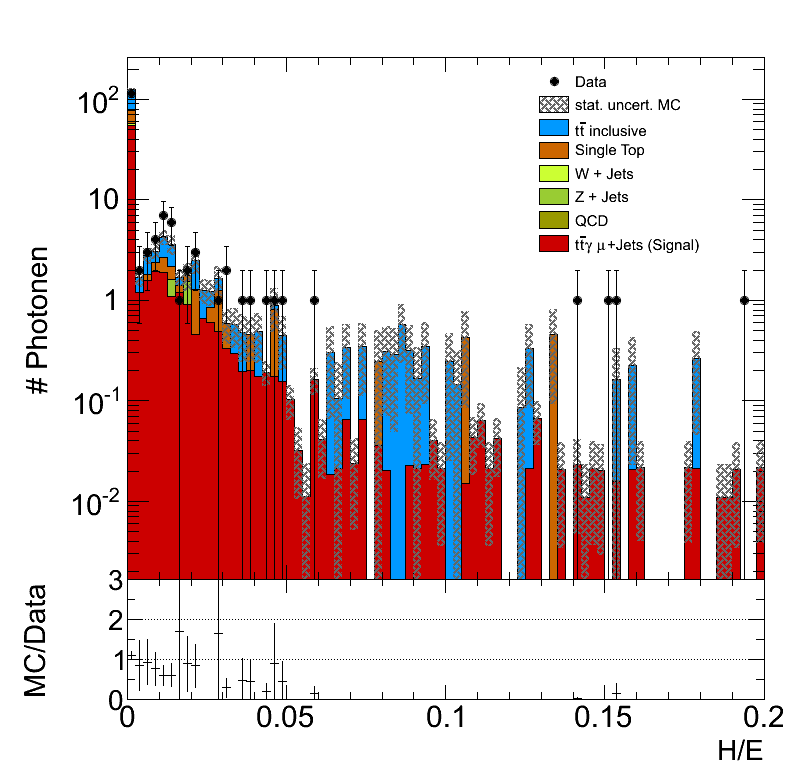
\includegraphics[width=\textwidth]{bilder/hadronicoverem_log}%
\end{subfigure}
\caption{$H/E$-Verteilung des Photons in linearer (links) und halblogarithmischer (rechts) Auftragung. Forderung: $H/E < 0,05$.}%
\label{fig:hadronicoverem_cut}%
\end{figure}

\begin{figure}%
\centering
\begin{subfigure}[b]{0.48\textwidth}
  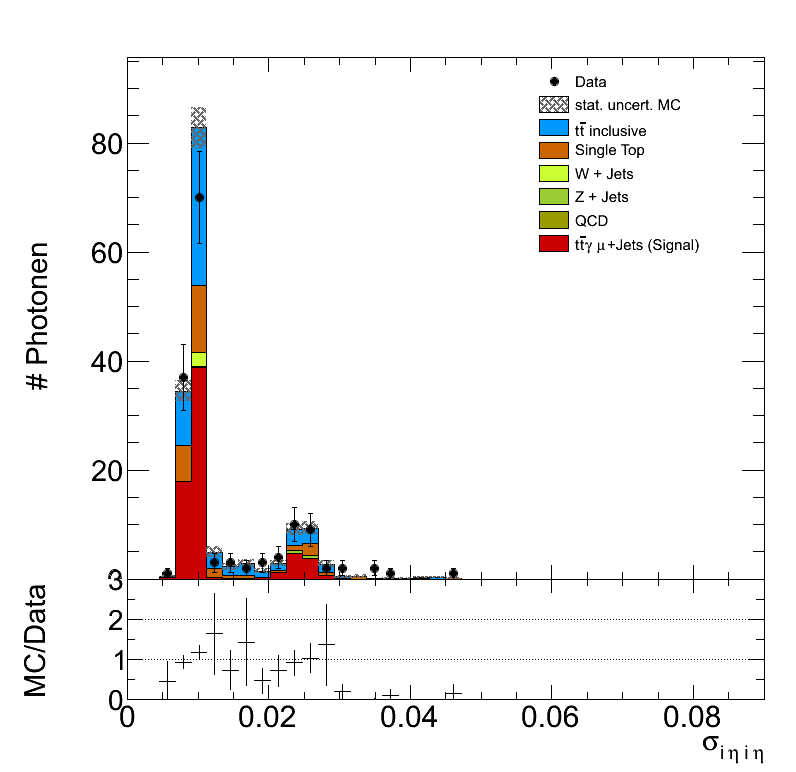
\includegraphics[width=\textwidth]{bilder/sigmaietaieta_linear}%
\end{subfigure}
\begin{subfigure}[b]{0.48\textwidth}
  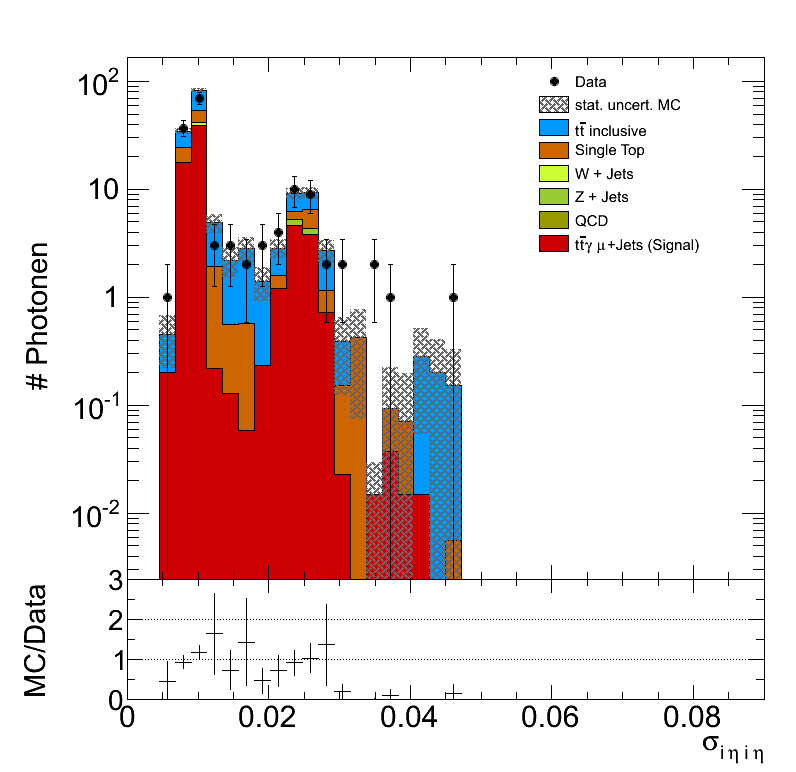
\includegraphics[width=\textwidth]{bilder/sigmaietaieta_log}%
\end{subfigure}
\caption{$\sigma_{i\eta i\eta}$-Verteilung des Photons in linearer (links) und halblogarithmischer (rechts) Auftragung. Forderung: $\sigma_{i\eta i\eta}<0,011$ im Bereich von $\left|\eta\right|<1,5$ und $\sigma_{i\eta i\eta}<0,03$ f�r $\left|\eta\right|>1,5$.}%
\label{fig:sigmaietaieta_cut}%
\end{figure}
